% Ensure that you compile using XeLaTeX !!! PDFTex has problems with some of the packages used
\documentclass[12pt]{article}
\setlength\parindent{0pt}

\usepackage{parskip}
\usepackage[margin=0.5in]{geometry}
\usepackage{fullpage}
\usepackage{moresize}
\usepackage{graphicx}
\usepackage{caption}
\usepackage{subcaption}
\usepackage{float}
\usepackage{xcolor}
\usepackage{soul}
\usepackage{fontspec}
\setmainfont{Doulos SIL}

\begin{document}

\begin{center}
\textbf{{\color{violet}{\HUGE 20201103 Tuesday\\}}}

\textbf{{\color{violet}{\HUGE ALL EXAMS\\}}}

\end{center}
\newpage

\begin{center}
\textbf{{\color{blue}{\HUGE START OF EXAM\\}}}

\textbf{{\color{blue}{\HUGE Student ID: 43803\\}}}

\textbf{{\color{blue}{\HUGE 4:00\\}}}

\end{center}
\newpage

{\large Question 1}\\

Topic: Articulatory Phonetics\\
Source: Homework 1, Question 3(a)\\

Could this image be the result of producing the sound represented by the given IPA symbol? Why or why not?\\

{[t͡ʃ]}

\begin{figure}[H]
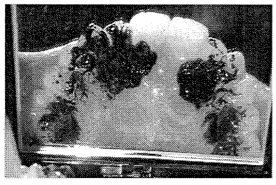
\includegraphics{../images/staticpalatography_fricative.png}
\end{figure}

\newpage

{\large Question 2}\\

Topic: Skewed Distributions\\
Source: Week 5 Handout, Question 3\\

What evidence is there that there is a pattern in these data, assuming that these are the only CV and VC sequences that occur in some language?\\

{[sa]}, {[ʃi]}, {[za]}, {[ʒi]}, {[as]}, {[iʃ]}, {[az]}, {[iʒ]}


\newpage

\begin{center}
\textbf{{\color{red}{\HUGE END OF EXAM}}}\\

\end{center}
\newpage

\begin{center}
\textbf{{\color{blue}{\HUGE START OF EXAM\\}}}

\textbf{{\color{blue}{\HUGE Student ID: 18870\\}}}

\textbf{{\color{blue}{\HUGE 4:10\\}}}

\end{center}
\newpage

{\large Question 1}\\

Topic: Articulatory Phonetics\\
Source: Quiz 2, Question 6\\

In the pronunciation of this word, which sounds are obstruents and which are sonorants? Explain your answer.\\

<language>


\newpage

{\large Question 2}\\

Topic: Transcription\\
Source: Week 2 Handout, Part II\\

Is this a reasonable transcription of this word? Explain why.\\

<choose>: {[t͡ʃuz]}


\newpage

\begin{center}
\textbf{{\color{red}{\HUGE END OF EXAM}}}\\

\end{center}
\newpage

\begin{center}
\textbf{{\color{blue}{\HUGE START OF EXAM\\}}}

\textbf{{\color{blue}{\HUGE Student ID: empty\\}}}

\textbf{{\color{blue}{\HUGE 4:20\\}}}

\end{center}
\newpage

\begin{center}
\textbf{{\color{blue}{\HUGE START OF EXAM\\}}}

\textbf{{\color{blue}{\HUGE Student ID: 28926\\}}}

\textbf{{\color{blue}{\HUGE 4:30\\}}}

\end{center}
\newpage

{\large Question 1}\\

Topic: Phonological Features\\
Source: Quiz 3, Question 12\\

Explain how you figure out which feature is involved in the process of umlaut shown below.\\

\begin{figure}[H]
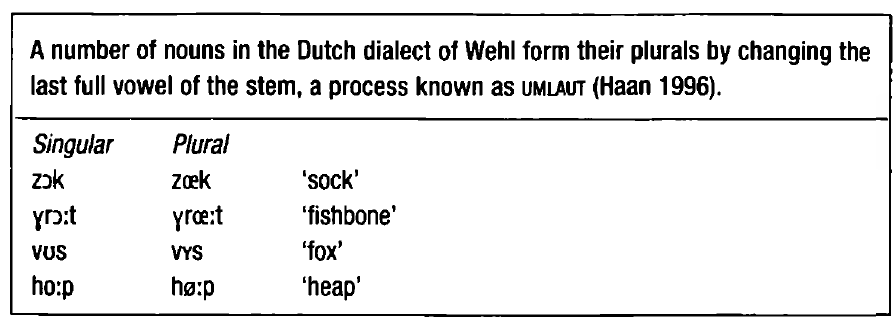
\includegraphics{../images/dutch.png}
\end{figure}

\newpage

{\large Question 2}\\

Topic: Articulatory Phonetics\\
Source: Homework 1, Question 3(b)\\

Explain why this is or is not a complete phonetic natural class in standard North American English.\\

{[ɔ]}, {[ʊ]}, {[u]}, {[oʊ]}


\newpage

\begin{center}
\textbf{{\color{red}{\HUGE END OF EXAM}}}\\

\end{center}
\newpage

\begin{center}
\textbf{{\color{blue}{\HUGE START OF EXAM\\}}}

\textbf{{\color{blue}{\HUGE Student ID: 83324\\}}}

\textbf{{\color{blue}{\HUGE 4:40\\}}}

\end{center}
\newpage

{\large Question 1}\\

Topic: Transcription\\
Source: Week 2 Handout, Part II\\

Is this a reasonable transcription of this word? Explain why.\\

<choose>: {[t͡ʃuz]}


\newpage

{\large Question 2}\\

Topic: Articulatory Phonetics\\
Source: Quiz 2, Question 7\\

Why might more than one of the descriptions given truthfully apply to the sound represented by the underlined letter, and why is one of them actually better than the other?\\

<a\underline{w}ay>

\begin{itemize} \item prevocalic obstruent \item prevocalic sonorant \item postvocalic obstruent \item postvocalic sonorant \item intervocalic obstruent \item intervocalic sonorant \end{itemize}


\newpage

\begin{center}
\textbf{{\color{red}{\HUGE END OF EXAM}}}\\

\end{center}
\newpage

\begin{center}
\textbf{{\color{blue}{\HUGE START OF EXAM\\}}}

\textbf{{\color{blue}{\HUGE Student ID: 80815\\}}}

\textbf{{\color{blue}{\HUGE 4:50\\}}}

\end{center}
\newpage

{\large Question 1}\\

Topic: Other (pre-midterm)\\
Source: Week 5 \& 6 Handouts\\

Explain how you could analyze this dataset in terms of sequential patterns vs. paradigmatic patterns.\\

\begin{figure}[H]
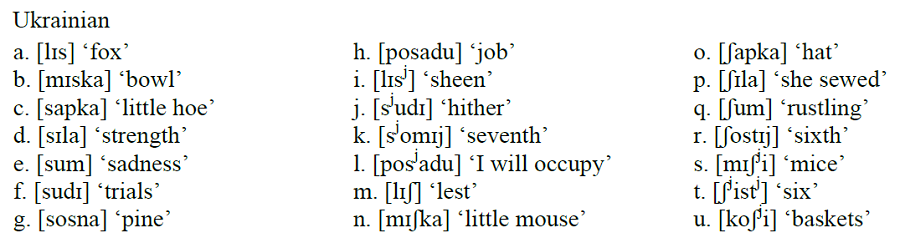
\includegraphics{../images/ukrainian.png}
\end{figure}

\newpage

{\large Question 2}\\

Topic: Skewed Distributions\\
Source: Week 5 Handout, Question 6\\

What would be a good description of the pattern in Malto? What characteristics make that a good description?\\

\begin{figure}[H]
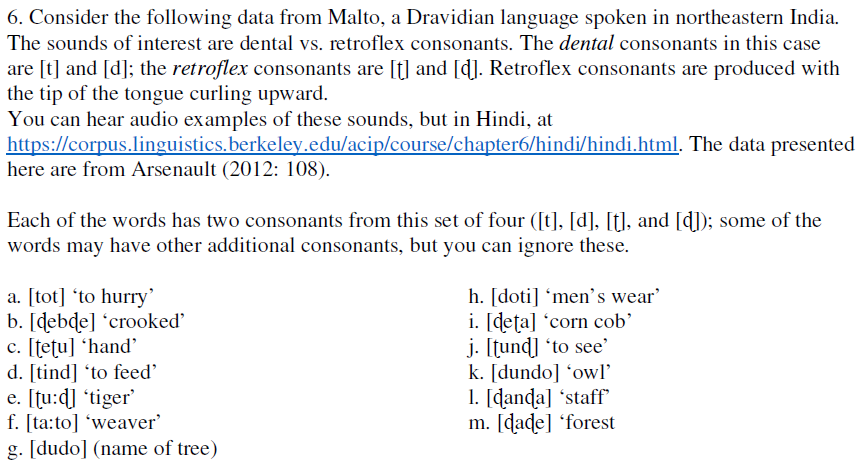
\includegraphics{../images/malto.png}
\end{figure}

\newpage

\begin{center}
\textbf{{\color{red}{\HUGE END OF EXAM}}}\\

\end{center}
\newpage

\end{document}

